\documentclass[a4paper,11pt,twoside]{article}

\usepackage[utf8]{inputenc}
\usepackage{amsmath,amsthm,amssymb}
\usepackage{mathtext}
\usepackage[T1,T2A]{fontenc}
\usepackage[english, russian]{babel}
\usepackage{graphicx}
\usepackage{url}
\usepackage{float}

\pagestyle{plain}

\title{\textbf{Правила для игры SAGA}\\ {\normalsize (Второе издание)}}
\author{Автор: Alex Buchel\\
		\\
		Неофициальный перевод: Александр Березовой \\
		(специально для клуба "Сквозь века" )}
\date{}
\begin{document}
\maketitle
\newpage
\tableofcontents
\newpage


\part*{Твоя Сага начинается здесь}
\addcontentsline{toc}{part}{Твоя сага начинается здесь}

\begingroup
	\fontsize{13pt}{11pt}\selectfont
	\textbf{\textit{Сага позволяет тебе как воссоздать ожесточённые сражения, проходившие между реальными враждующими народами в разные исторические эпохи, так и окунуться в битвы из фэнтези миров. В этот век героев храбрые воины встретятся на поле боя, ведомые твоими инстинктами и тактической смекалкой (с небольшой долей рассчёта на удачу, конечно же!)! \\
	Пришло время вписать своё имя на страницы истории. Пусть сталь будет твоим пером, а кровь - чернилами...}}
\endgroup

\section*{Добро пожаловать в Сагу}

Книга, которую ты держишь в своих потных трясущихся ладошках, - главный ключ к тому, чтобы начать играть во многих вселенных. Она содержит основные правила к игре с миниатюрами SAGA и фундаментальные принципы игры, которые будут работать вне зависимости от того, какой исторический период или какую вселенную ты выберешь для игры. Скоро ты поймёшь, что правила просты и легко усваиваются, но содержат в себе вещи, для осознания которых требуется время. Для ускорения твоего обучения правила содержат в себе много советов и примеров того, как играть в эту игру.\\ \\
Помимо ядра игры, которое ты прямо сейчас держишь в своих руках, тебе понадобится Вселенная Саги. Какие-то вселенные уже доступны для игры, другие же появятся позже. Ты можешь играть в Эпоху Викингов, Век Крестовых Походов, Эру Короля Артура и многие другие. Вселенная, которую ты выберешь, должна удовлетворять твоим вкусам и желаниям, а также тому набору фигурок, который у тебя есть. (Запомни, это касается и тех бравых ребят, с которыми ты будешь играть!). Правила в этой книге будут работать для любой вселенной.\\ \\
Тебя страшат мысли о боевом вожде на поля боя, окружённом всё ещё тёплыми мертвецами и с кровавой сталью в руках?! Если нет, то Сага покажется тебе не страшнее, чем чашечка горячего чая. Ну а если тебе страшно, то мы можем посоветовать только выбрать более мирное хобби. Например, шитьё. 
\newpage
\begingroup
\fontsize{15pt}{11pt}\selectfont
\textit{Книжник поможет тебе...}\\ \\
\fontsize{11pt}{11pt}\selectfont
\textit{Я Книжник, тот, кто без устали ведёт летопись хроник Вселенных Саги и тот, кто будет вести тебя на этих страницах. Время от времени я буду давать тебе советы, которые пригодятся тебе вне зависимости от эры, в которой ты играешь. Никогда не забывай их, ведь даже перед лицом самой страшной опасности хладнокровие это всё, что стоит между героем и его могилой!}
\endgroup 
\section*{Что тебе понадобится для игры}
Давай же немедленно перейдём к списку того, что тебе понадобится для игры. \\ \\
Для начала, так как Сага - игра с миниатюрами, тебе понадобятся миниатюры, модели солдат. Каждый игрок является лидером отряда, военного формирования или, как принято говорить среди некоторых игроков, \textbf{банды}, численностью в среднем от 20 до 50 фигурок. Размер фигурок не важен, но по иллюстрациям в этой книге ты поймёшь, что мы предпочитаем играть миниатюрами высотой 28мм, хотя финальный выбор всё равно за тобой. Мы ещё не готовы выпустить наши карательные отряды ''Чистая Сага'', чтобы следить за тем, что игроки делают с нашими продуктами. \\ \\
Также тебе понадобится поверхность, на которую ты поставишь свои замечательные фигурки. Стандартное игровое поле саги имеет размеры: 120см на 90см (или 48 на 36 дюймов). Поле было специально сделано так, чтобы у игроков было место, куда поставить еду и напитки, которые так необходимы во время свирепой схватки! \\ \\
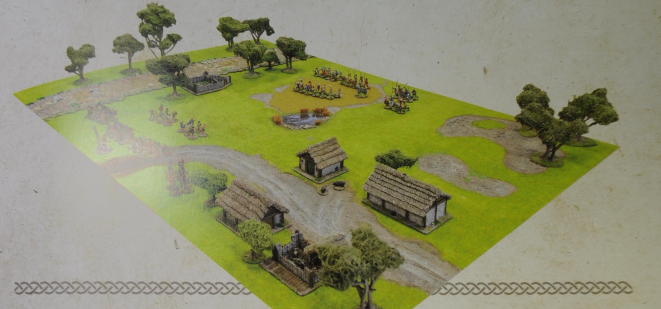
\includegraphics[width=1.0\textwidth]{pics/SagaBoard} \\ \\ \\
Украшающие твою доску декорации также важны - зоны, которые они занимают, могут влиять непосредственно на сам процесс игры. В самом простом случае деревья могут быть представлены в виде схематичного рисунка или контура на доске, но, честно говоря, если ты будешь использовать модели деревьев для этого, игра не станет хуже, скорее, наоборот! \\ \\
Для измерения расстояний тебе понадобятся четыре измерительные линейки определённой длины. В Саге используется 4 единицы измерения длины: \begin{itemize}
\item Very Short (Очень короткая), обозначается \textbf{VS} и равна 2 дюймам
\item Short (Короткая), обозначается \textbf{S} и равна 4 дюймам
\item Medium (Среднее), обозначается \textbf{M} и равна 6 дюймам
\item Long (Длинная), обозначается \textbf{L} и равна 12 дюймам 
\end{itemize}
Существуют официально продаваемые линейки, но вы можете сделать свои собственные по шаблонам, доступным на нашем сайте (\url{www.studio-tomahawk.com}). Помни, что эти линейки - единственное реальное оружие, участвующее в игре, так что убедись в том, что они вселят ужас в оппонента и дадут тебе психологическое преимущество! \\ \\
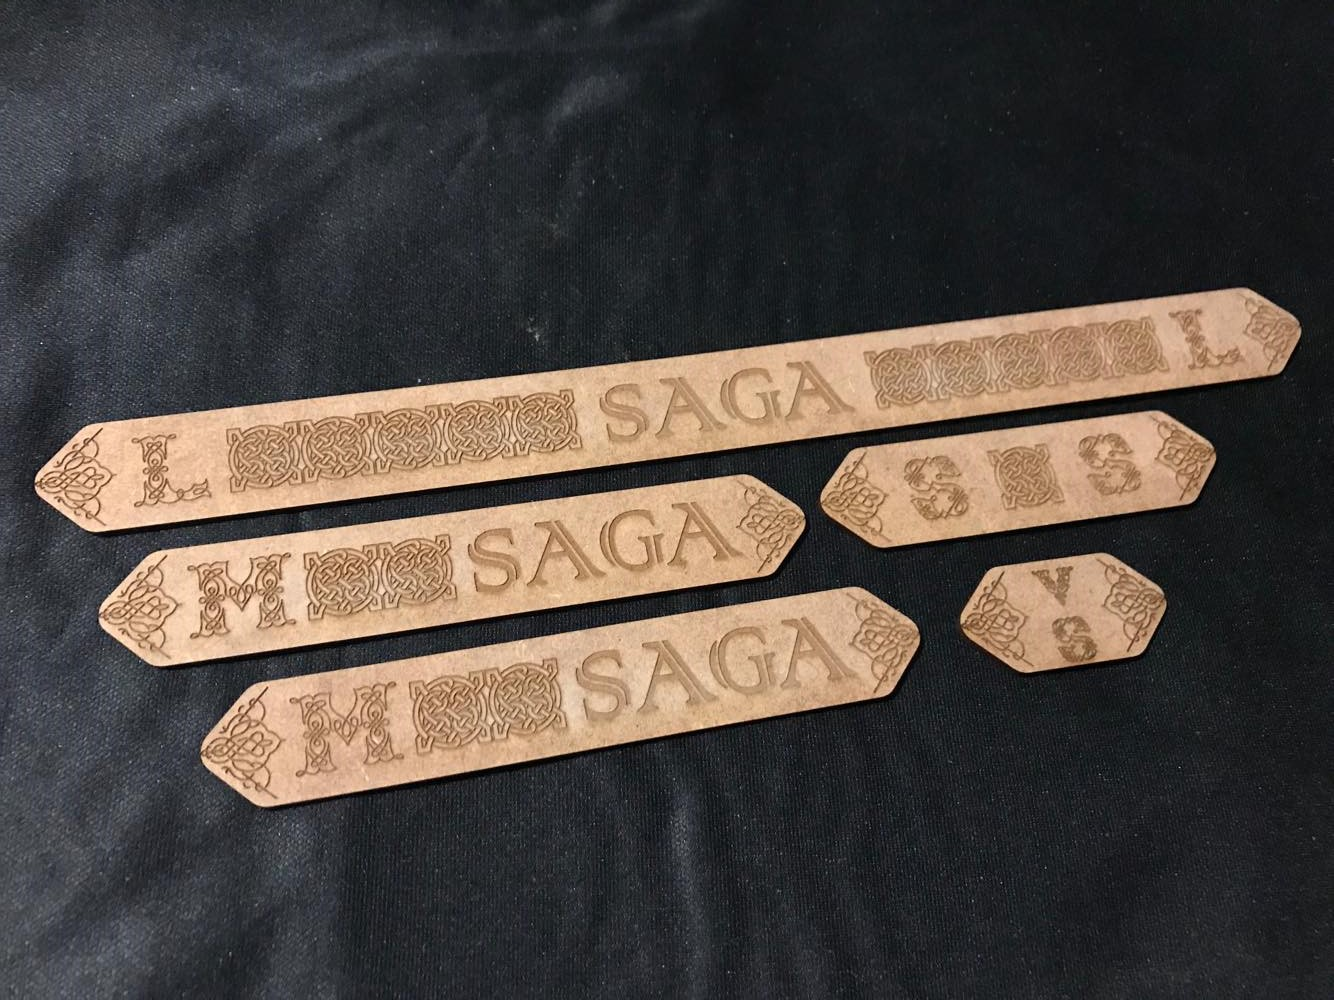
\includegraphics[width=1.0\textwidth]{pics/SagaSticks} \\ \\ \\
Так как игрокам всегда нужно что-то, на что они злятся, когда Леди Удача отворачивается от них, Сага использует два типа кубов. Первый - это старые-добрые шестигранные кубики, которые легко достать и которых полным-полно у бывалых варгеймеров. Второй тип это кубики Саги. Это шестигранные кубики, на гранях которых начертаны особые символы. На данный момент существует достаточно много типов кубов Саги, которые вы можете купить либо же сделать сами. Каждому игроку понадобится 8 кубов Саги своей фракции для игры. Тип кубов Саги для каждой фракции указан в соответствующей книге правил и нарисован на боевой доске фракции. \\ \\
Наконец, тебе понадобятся жетоны для обозначения \textbf{усталости} - наказания для тех, кто сражается слишком долго или совершает немыслимые подвиги. Опять же, ты можешь купить эти жетоны или сделать сам.
\part{Основы}
\textbf{\textit{В этой главе мы разберёмся со многими элементами игры и некоторыми общими правилами }} \\ \\ \\
\textit{Примечание переводчика: в данной книге в равном значении будут использоваться понятия \textbf{банда, военное формирование, военная банда, армия и т.п.}. Под этим словом я подразумеваю все фигурки и юниты, подконтрольные игроку во время сражения.}
   \section*{Отряды и фракции}
В Саге каждый игрок управляет \textbf{бандой}, численность которой, как мы видели ранее, составляет около тридцати миниатюр. Эта банда является частью \textbf{фракции}, которая представляет реальные исторические народы, фэнтези-расу (например, орки) или персонажей мифологии (Аргонавты). Каждая фракция является частью какой-то Вселенной Саги и детально описано в соответствующей книге правил. \\ \\ 
У каждой фракции есть собственная \textbf{боевая доска} (батлборд). Это не та доска, которой ты избиваешь своего оппонента, а специальный лист картона, на котором изображены способности твоей фракции. Как мы увидим далее, именно боевая доска и кубики Саги - самый сок этой игры! \\ \\ 
Система очков набора фигурок призвана сделать сражения сбалансированными, а банды равными. Сражения Саги играются армиями, собранными на количество очков между 4 и 8. Обычно игроки выбирают формат 6 очков, но мы тебе советуем свои первые игры проводить на 4 очка, чтобы быстрее ознакомиться с механикой игры. Каждое очко позволяет тебе набрать определённое количество фигурок (см. главу "Сбор армии"). \\ \\ 

\subsection*{Типы солдат}
В Саге каждая фигурка принадлежит одному из четырёх типов солдат, описанных ниже.

\subsubsection*{Герои}
Герои - главные и самые яркие представители каждой эпохи Саги. Они сами по себе считаются \textbf{подразделениями} и обладают способностями, которые превосходят возможности простых смертных. Именно они рождают легенды. \\ \\
В частности, один герой всегда ведёт за собой любую банду - это ваш \textbf{Боевой Вождь (Варлорд)}. Он бывалый воин, хитроумный и могущественный, всегда готовый ворваться в гущу сражения. Своего рода фентезийное альтер-эго для большинства игроков! \\ \\
Другие герои описываются в каждой отдельно взятой Вселенной Саги - они могут быть историческими личностями, волшебниками или легендарными существами. \\ \\
\subsubsection*{Воины правителя} 
Воины правителя - это лучшие бойцы в твоём распоряжении, они представляют собой хорошо обученных солдат с лучшим из доступного снаряжением. Как правило, составляют личную охрану для Боевого Вождя и Героев. Это именно те парни, которых стоит звать с собой в таверну!
\\ \\
\textit{Примечание переводчика: альтернативный перевод - Дружина правителя, Дружина, Дружинники}
\subsubsection*{Воины}

Воины - это основа любой армии. Обыкновенные солдаты, которые что-то смыслят в ратном деле и вооружены, возможно, не самым лучшим, но всё ещё опасным оружием. Воины редко носят броню и больше полагаются на численность как в атаке, так и в обороне. Если столкнёшься с ними в двери таверны, лучше посчитай, сколько их, прежде чем лезть в драку.

\subsubsection*{Рекруты}

Они никогда этого не хотели, но драться им придётся - Боевой Вождь заставит! Он полагается на их огромную численность и в каждой битве старается избавиться от своих самых жалких слуг, не утруждая себя судами и бумажной волокитой. Если они попадутся тебе на пути в таверне - отправь смердов принести тебе пиво!

\subsection*{Характеристики}

В Саге у фигурок имеется две характеристики: Броня и Агрессия.  \\ \\
Броня представляет собой качество защитного снаряжения и то, как тяжело противнику будет вывести воина из боя. В зависимости от того, как они снаряжены, фигурки могут иметь разные показатели Брони в ближнем бою и против дальних атак. Броня не может быть меньше значения "2" и больше значения "6". \\ \\
Агрессия - это то, сколько кубиков получает \textbf{подразделение} во время атаки. Агрессия имеет разные значения для ближнего и дальнего боя и может быть представлена как целым числом, так и дробью. \\ \\ 
Эти характеристики одинаковы для того типа солдат, которому принадлежит фигурка. То есть, все Воины Правителя имеют одинаковую Броню и Агрессию, это же справедливо для Воинов и Рекрутов. \\ \\
В отличие от Боевых Вождей, у которых тоже эти характеристики совпадают, Герои являются исключением, и их Броня и Агрессия варьируются в зависимости от конкретного Героя. \\ \\
Снаряжение, носимое фигуркой, может менять эти характеристики. Например, лучник жертвует своей Бронёй, чтобы ему было легче управляться с луком. \\ \\

\subsection*{Подразделения}

Каждая фигурка принадлежит своему \textbf{подразделению}, которое на начало игры включает в себя от 4 до 12 фигурок - ни больше, ни меньше. Внутри одного подразделения все фигурки должны быть одного типа (Воины правителя, Воины, Рекруты) и иметь одинаковое снаряжение. Подразделение не может разделено или объедено с другим подразделением во время игры. \\ \\ 

\textit{Примечание переводчика} \\
\textit{Часто будет встречаться термин ''юнит'', это то же самое, что и подразделение.} \\ \\

Герои (будь они неладны!) являются исключением. Они составляют подразделение численностью в одну фигурку и, если это не указано дополнительно, не могут сопровождаться другими фигурками. \\ \\ 

\begingroup
\fontsize{15pt}{11pt}\selectfont
\textit{Книжник поможет тебе...}\\ \\
\fontsize{11pt}{11pt}\selectfont
\textit{Довольно часто фанаты Саги ставят вместе с героем на большую подставку другие фигурки - слуг, пажей или питомцев Героя. Эти фигурки носят чисто декоративный характер и подставка с Героем считается одной фигуркой в рамках правил игры.}
\endgroup 

\subsection*{Построения}

Во время своего размещения или по окончанию движения подразделение должно удовлетворять некоторым правилам построения. \\ \\
Во-первых, каждая фигурка должна находиться не дальше, чем на дистанции \textbf{VS} от другой фигурки своего подразделения. Это значит, что если провести ломаную линию между всеми фигурками одного юнита, не будет промежутка длиннее, чем \textbf{VS}. Ты никогда не можешь нарушать это правило: ни когда убираешь фигурки из-за боевых потерь, ни в каких других случаях. \\ \\ 
Во-вторых, после размещения или по окончанию движения, расстояние от первой двигавшейся или выставленной фигурки до любой другой фигурки подразделения должно быть не больше, чем \textbf{S}. Это означает, что все фигурки подразделения должны помещаться в воображаемый круг радиуса \textbf{S} с первой фигуркой в центре. Для конных юнитов данное правило работает иначе (см. соответствующую главу). \\ \\
Заметь, что в Саге то, куда смотрит фигурка, не влияет на игру. Мы всё равно советуем тебе ставить твои фигурки лицом к противнику, чтобы избежать язвительных комментариев от тех, кто будет наблюдать за битвой. \\ \\ 

\subsubsection*{Подставки}

Фигурки в Саге должны находиться на подставках, которые могут быть в форме прямоугольника, круга или какой угодно, решает игрок. Однако они всё же должны удовлетворять следующим критериям:
\begin{itemize}
\item Подставка верховой фигурки должна помещаться в квадрат со стороной 50мм и не может быть меньше, чем прямоугольник со сторонами 40мм и 20мм
\item Подставка пешей фигурки должна помещаться в квадрат со стороной 30мм и не может быть меньше, чем квадрат со стороной 20мм
\item Подставка Героя, неважно, пешего или верхового, должна помещаться в квадрат со стороной 60мм. Минимальный размер зависит от того, пеший Герой или на коне и удовлетворяет критериям, описанным выше для обычных миниатюр.
\end{itemize} 
Минимальный диаметр круглой подставки и минимальная ширина прямоугольной является 20мм. \\ \\

\section*{Принципы игры}

Здесь будут описаны некоторые элементы, которые проиллюстрируют основные принципы игры. Ты должен будешь помнить их, читая остальную часть правил.

\subsection*{Ход}

Игра в Сагу идёт некоторое количество ходов, передаваемых между игроками. Ход игрока разделён на две фазы: Фазу Приказов, во время которой игрок бросает свои кубики Саги и выставляет их на Боевой Доске, и Фазу Активаций, во время которой подразделения действуют согласно тому, как игрок распределил кубики в прошлую фазу. Как только Фаза Активаций игрока заканчивается, его ход завершён и начинается ход его противника. \\ \\ 

\subsection*{Сценарии}

Любая игра в Сагу идёт согласно сценарию, который определяет условия победы, то, как расставляются юниты на поле боя, любые специальные правила и количество ходов. \\ \\
В конце книги ты найдёшь базовый сценарий, который направит тебя на путь воина безжалостных земель мира Саги - "Противостояние Боевых Вождей". Дополнительный набор Саги, "Book of battles"  содержит большое количество других сценариев, описывающих более интересные и необычные ситуации. \\ \\

\subsection*{Измерения}

Как мы упоминали до этого, в игре 4 вида измерений. \\ \\

\begin{itemize}
\item Very Short (Очень короткая), обозначается \textbf{VS} и равно 2 дюймам
\item Short (Короткая), обозначается \textbf{S} и равно 4 дюймам
\item Medium (Среднее), обозначается \textbf{M} и равно 6 дюймам
\item Long (Длинная), обозначается \textbf{L} и равно 12 дюймам 
\end{itemize} 

В этой книге, как и во всех остальных материалах Саги, мы будем пользоваться этими обозначениями - так что запомни их побыстрей! Например, будет сказано, что дальность стрельбы из лука равна L, и не будет сказано, что лук стреляет на 12 дюймов.
\\ \\ 
Сага разрешает тебе выполнять измерения в любое время, в любой ситуации. То есть, до того как скомандовать стрельбу, ты можешь убедиться, что все твои фигурки достают до противника - и наоборот, перед тем, как получить залп стрел противника в брюхо, ты можешь измерить расстояние от атакующих до своих бравых ребят. \\ \\ 
Часто будет всплывать термин "\textit{быть на дистанции X}". X может быть VS, S, M или L. Для подразделения, фигурки или декорации ''\textit{быть на дистанции X}'' означает, что достаточно части подразделения, фигурки или декорации быть на расстоянии X или меньше, чтобы выполнилось это условие. \\ \\ 
\textit{\textbf{Заметьте, что достаточно части подставки фигурки из подразделения быть на дистанции X, чтобы всё подразделение считалось находящимся на дистанции X}} \\ \\
Единственное исключение из этого правила - формулировка ''\textit{Полностью внутри X}'', ''\textit{В пределах X}'', которое означает, что всё подразделение или декорация должна лежать на дистанции X. \\ \\ 

\begingroup
\fontsize{15pt}{11pt}\selectfont
\textit{Книжник поможет тебе...}\\ \\
\fontsize{11pt}{11pt}\selectfont
\textit{Высказывать своё намерение очень важная часть игры в Сагу, которая помогает избежать лишних споров и бесконечных склок. Если ты двигаешь своё подразделение, собираясь увести его из-под огня вражеских лучников, сообщи своему противнику, что ты остаёшься на дистанции дальше L. Тогда во время его хода, даже если крошечная часть подставки фигурки из твоего подразделения находится в пределах L, ситуация быстро может быть решена небольшими подвижками, ссылаясь на то, что ты сообщил о своём намерении до этого. Так мы в Саге избегаем лишнего кровопролития.}
\endgroup 

\subsection*{Перебросы и модификаторы}

Некоторые игровые эффекты позволят тебе перебросить кубик (сейчас речь идёт о стандартном шестигранном кубике, D6). Игрок может перебросить каждый кубик только один раз за ход и обязан оставить результат, полученный после переброса, даже если этот результат хуже изначального. \\ \\ 
Результат, выпавший на кубике, может быть изменён как в большую, так и в меньшую сторону (например, +1 или -2). Любой результат после модификации, который численно меньше 0, считается равным 0, но при этом верхняя граница может превосходить 6. Например, бросок кубика на 5, модифицированный на +2, даст тебе в результате 7. \\ \\ 
Эти правила не применяются к Кубам Саги, которые могут быть переброшены сколько угодно раз и у которых нет никаких численных значений. \\ \\ 

\subsection*{Дроби}

Сага с завидной регулярностью использует дробные значения - как слова (половина, треть и т.д.), так и числовой эквивалент (1/2, 1/3 и т.д.). \\ \\ 
Во всех случая применяется простое правило: дроби округляются вверх до ближайшего целого. Например, если треть твоего отряда из восьми фигурок внезапно захочет справить нужду в ближайших кустах, то три воина из восьми поддадутся зову природы, пока враг не видит. \\ \\ 

\subsection*{Давид против Голиафа}

Временами в Саге случается так, что разные правила или способности начинают противоречить друг другу и создают неразрешаемые ситуации. Довольно обычной является момент, когда способность требует от отряда сделать что-то, когда другая способность не даёт. В таких ситуациях работает следующее правило - запрет побеждает необходимость - ''не может'' главнее ''должен''. \\ \\ 


\begingroup
\fontsize{15pt}{11pt}\selectfont
\textit{\textbf{Что ты должен запомнить}}\\ 
\fontsize{11pt}{11pt}\selectfont
\begin{itemize}
\item У каждого подразделения есть тип: Герой, Воин правителя (Дружинник), Воин или Рекрут.
\item Юниты (подразделения) Саги, за исключением Героев, состоят из 4-12 фигурок.
\item В любой момент можно измерять любое расстояние до чего-либо.
\item Во время игры противники ходят по очереди.
\item Ход делится на две фазы: Фаза Приказов и Фаза Активаций.
\item Дроби всегда округляются вверх до ближайшего целого.
\end{itemize}
\endgroup 
\newpage
\part{Фаза приказов}
\textbf{\textit{Как мы увидели, ход состоит из двух идущих друг за другом фаз: Фаза Приказов и Фаза Активаций. Эта глава описывает первую, и, по мнению ветеранов Саги, самую важную фазу: Фазу Приказов. }} 
\section*{Боевые Доски и Кубы Саги}
У каждой фракции своя Боевая Доска (ты найдёшь их в той Вселенной Саги, которую выберешь для игры), которая используется вместе с соответствующим набором Кубов Саги. \\ \\ 
Ниже пример Боевой Доски и краткая информация о её содержании
\newpage
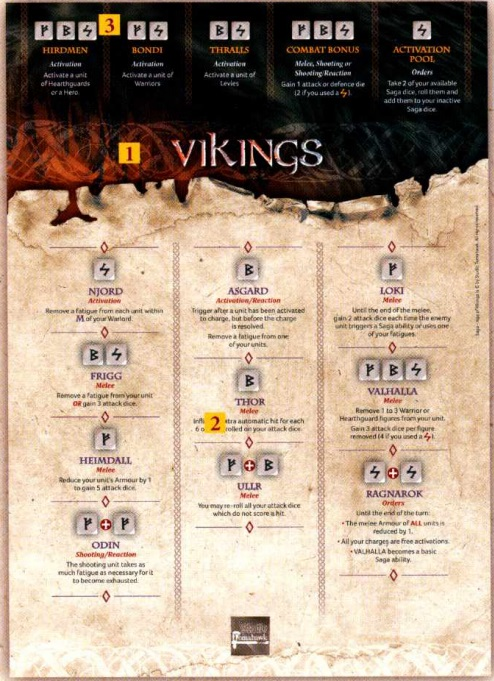
\includegraphics[width=1.0\textwidth,]{pics/SagaBattleboard} \\ \\ \\
\begin{enumerate}
\item Название фракции
\item Умения Саги этой фракции. В общем случае, здесь 15 умений: одни расположены выше названия фракции, другие ниже. Позже мы увидим, в чём разница между ними, а пока что запомни, что умения Саги позволяют подразделениям совершать действия во время игры.
\item Кубик Саги, который нужен тебе для игры этой фракцией. На каждом умении Саги нарисован результат броска, который необходим для активации этого умения.
\end{enumerate} 
Боевая Доска (Батлборд) используется вместе с Кубами Саги. В начале каждого хода ты кидаешь определённое количество Кубов Саги и расставляешь их на умения Саги на батлборде. \\ \\ 
Все Кубы из одного набора одинаковы. Они устроены так, что один из символов расположен на трёх гранях, один на двух и последний присутствует только на одной грани. \\ \\ 
Ты играешь с \textbf{восемью} Кубами Саги - ни меньше, ни больше. Иметь больше восьми Кубов всё равно что хранить туз в рукаве во время покерной партии. \\ \\ 
\subsection*{Фаза приказов}
Во время фазы приказов ты планируешь действия, которые совершишь в Фазу Активаций. Фаза происходит следующим образом:
\begin{itemize}
\item Брось столько Кубов Саги, сколько генерирует твоя боевая банда
\item После этого ты должен позволить противнику сыграть \textbf{умения-реакции}
\item Теперь ты можешь расставить Кубы на умения и \textbf{задействовать} умения, которые работают в Фазу Приказов, меня очерёдность по своему усмотрению.
\item Ещё раз позволь своему противнику сыграть \textbf{умения-реакции}.
\end{itemize}

\begingroup
\fontsize{15pt}{11pt}\selectfont
\textit{Книжник поможет тебе...}\\ \\
\fontsize{11pt}{11pt}\selectfont
\textit{Когда противник играет умения-реакции, он задействует способности, которые разрушают твои грандиозные планы. Стоит привыкать к этому очень быстро - противники, которые позволяют тебе делать то, что ты хочешь, вещь редкая!}
\endgroup 

\section*{Генерация Кубов Саги}

В начале Фазы Приказов ты должен выяснить, сколько Кубов ты можешь бросить. Здесь нет ничего сложного. \\
Возьми \textbf{по одному} Кубу за:
\begin{itemize}
\item твоего Боевого Вождя, если он ещё на поле
\item каждое подразделение Дружинников, которое ещё на поле
\item каждое подразделение Воинов, находящееся на поле и содержащее по меньшей мере 4 фигурки
\item каждое подразделение Рекрутов, находящееся на поле и содержащее по меньшей мере 6 фигурок
\end{itemize}

Добавь к этим Кубам:
\begin{itemize}
\item Кубы, сгенерированные другими твоими Героями, находящимися на поле. Каждый Герой генерирует разное количество Кубов Саги, которое ты найдёшь в описании Героя. 
\end{itemize}

Временами твоя Боевая Банда будет генерировать больше, чем 8 Кубов Саги, но несмотря ни на что, в начале хода ты не можешь бросить больше, чем 8 Кубов Саги. \\ \\ 
\begingroup
\fontsize{15pt}{11pt}\selectfont
\textit{Книжник поможет тебе...}\\ \\
\fontsize{11pt}{11pt}\selectfont
\textit{Вообрази Мирмидонцев, собирающихся наброситься на своих врагов Троянцев. После первых обменов ударами у них остались: 
\begin{itemize}
\item Юнит из 6 Дружинников
\item Юнит из 2 Дружинников
\item Юнит из 10 Воинов
\item Юнит из 3 Воинов
\item Юнит из 9 Рекрутов
\item и Варлорд, смело ведущий их в бой.
\end{itemize}
На начало хода наш Ахиллес, играющий в Сагу, должен сгенерировать свои Кубы Саги. Он получает: 
\begin{itemize}
\item 1 Куб за 6 Дружинников
\item 1 Куб за 2 Дружинников
\item 1 Куб за 10 Воинов
\item 1 Куб за 10 Рекрутов
\item и 1 Куб за Варлорда.
\end{itemize}
Юнит из 3 Воинов не генерирует Куб Саги, потому что в нём меньше, чем 4 фигурки. Итого, игрок будет бросать 5 Кубов во время Фазы Приказов.}
\endgroup 

\section*{Бросок Кубов Саги}

Теперь, когда ты знаешь, сколько Кубов должен бросить, возьми их!
Возможна ситуация, когда у тебя остались Кубы Саги на Батлборде с прошлого хода. Такое случается, если ты положил Куб на способность, но по каким-то причинам не смог или не захотел использовать её. До броска Кубов, ты можешь снять какие-то Кубы с Батлборда. Это необходимо на тот случай, если тебе не хватает Кубов для броска сгенерированного в начале хода количества Кубов. \\ \\ 

\begingroup
\fontsize{15pt}{11pt}\selectfont
\textit{Книжник поможет тебе...}\\ \\
\fontsize{11pt}{11pt}\selectfont
\textit{Вообразим, что наши Мирмидонцы всё ещё имеют 4 Куба Саги на своём Батлборде. Они сгенерировали 5 Кубов Саги, но не смогут бросить все, если не уберут один Куб с Батлборда - помни, что каждый игрок имеет на руках ровно 8 Кубов Саги!}
\endgroup 

Как мы увидим далее, определённые умения Саги требуют для использования два Куба Саги. Если ты решишь убрать один Куб с такой способности, тебе придётся убрать оба Куба. Ты не можешь оставить часть Кубов, необходимых для активации способности, на доске, а часть забрать для броска. \\ \\ 
Когда ты закончишь, соверши бросок Кубов. До тех пор, пока Кубы не выставлены на Батлборд, они считаются \textbf{неактивными}. Те Кубы, которые ты ещё не бросил и которые ещё не выставлены на умения Саги, считаются \textbf{доступными}. \\ \\ 
Как только ты бросил Кубы, твой противник может задействовать свои \textbf{умения-реакции} (мы вернёмся к ним позже).

\section*{Расстановка Кубов Саги}

Теперь, когда ты совершил бросок Кубов Саги, у тебя есть несколько символов, которые совпадают с символами, изображёнными на умениях Саги, изображённых на Батлборде. Давай повнимательней посмотрим на умение Саги:

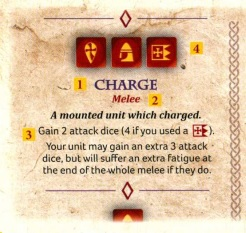
\includegraphics[width=1.0\textwidth]{pics/SagaPlacingDice.jpg}
\begin{enumerate}
\item Название умения.
\item Ключевое слово умения: это слово показывает, в какой момент игры данная способность может быть активирована. На рисунке у нас ключевое слово ''Ближний бой'', что означает, что ты можешь задействовать эту способность только во время рукопашной схватки. Определённые способности имеют несколько ключевых слов, что даёт тебе больше свободы относительно выбора момента, когда их задействовать.
\item Описание умения. Другими словами, что конкретно происходит в момент, когда способность активирована. Ограничения в использовании способности мог быть написаны \textit{курсивом} прямо перед ключевым словом. Например, некоторые умения могут быть использованы только для определённого типа солдат. Способность на рисунке может быть использована только конным юнитом, который совершил \textit{активацию на атаку}. Следовательно, твоя пехота не может использовать это умение.
\item Цена умения, изображённая символами на Кубах. Цена показывает Куб или Кубы, необходимые для активации умения. Мы рассмотрим этот аспект более подробно дальше.
\end{enumerate}

Те умения, которые расположены над названием фракции - это \textbf{базовые} умения. Под названием фракции расположены \textbf{специальные} умения. \\ \\ 
Базовые умения могут быть задействованы несколько раз за ход, в то время как специальные умения могут быть задействованы только один раз за ход. \\ \\ 
Временами в нижней части Батлборда будут появляться способности с ключевым словом \textbf{"Базовая"} ("Basic"). Такие способности так же могут быть задействованы несколько раз в ход. \\ \\ 
Каждая способность имеет цену, выраженную в Кубах саги. Это те символы, которые изображены над названием способности. \\ \\ 
Многие способности Саги дают тебе свободу выбора относительно того, какой Куб потратить. Например: \\ \\
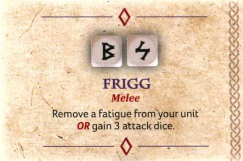
\includegraphics[width=1.0\textwidth]{pics/SagaSeveralDiceAbility} \\ \\ \\
Эту способность ты можешь активировать, выставив на неё любой из этих двух символов. Как только ты выставляешь Куб Саги на способность, она считается \textbf{активированной}, а выставленный Куб - \textbf{активным Кубом Саги}. \\ \\ 
Некоторые способности требуют два Куба, чтобы активироваться. В этом случае необходимые Кубы будут разделены знаком ''+'', как показано в примере ниже. \\ \\
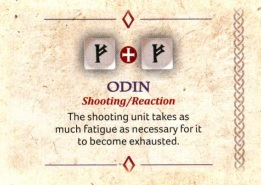
\includegraphics[width=1.0\textwidth]{pics/SagaMultipleDiceAbility} \\
Ты обязан поместить оба кубика одновременно. Ты не можешь поместить только один кубик и ждать, пока Госпожа Удача подарит тебе второй. \\ \\ 
Базовые способности ты можешь активировать несколько раз за ход, просто помещая на них несколько кубиков. Это значит, что ты можешь задействовать одну и ту же Базовую способность несколько раз за ход. Специальные же умения ты можешь активировать и задействовать только один раз за ход. Это означает, что ты можешь поместить только один кубик (или комбинацию, в случае способностей с двумя кубами) на такое умение в Фазу Приказов, и, следовательно, задействовать только один раз за ход. \\ \\
\section*{Задействование способностей Приказов}
Во время Фазы Приказов, ты можешь задействовать способности с ключевым словом \textbf{Приказы (Orders)}, даже если ты только что активировал их. Способности Приказов часто оказывают влияние на течение самой Фазы Приказов, так, например, они позволяют перебросить неактивные Кубы Саги или даже бросить дополнительные. В то же время такие способности могут иметь эффекты, действующие до конца хода. \\ \\
Чтобы \textbf{задействовать} способность, сними куб или кубики со способности, равные цене способности (в случае Базовой способности по одному кубику за применение). Снятые кубики убираются с Боевой Доски и считаются \textbf{доступными кубиками} (как будто бы ты не бросал их). Затем разыграй эффект умения. После этого ты можешь задействовать другую Способность Приказа или продолжить выставлять кубики. Продолжай до тех пор, пока не решишь, что ты сделал всё, что хотел в своей Фазе Приказов. \\ \\ 

\subsection*{Задействование способностей Саги}
\begin{itemize}
	\item Описание задействования способности Приказов применяется ко всем способностям Саги в игре (и мы увидим, что существуют другие виды способностей помимо Приказов). Чтобы задействовать способность, тебе просто надо снять необходимый кубик или кубики, отложить их к доступным кубам и разыграть эффект способности.
\end{itemize}

\section*{Конец Фазы Приказов}
Прямо перед тем, как закончить свою Фазу Приказов, ты должен дать своему противнику задействовать его умения-реакции Приказов. \\ \\
Когда это сделано, в том маловероятном случае, если у тебя остались неактивные кубики Саги (это те, которые ты бросил, но не поместил на Боевую Доску), они становятся доступными кубами Саги. \\ \\
На этом твоя Фаза Приказов кончается и начинается ключевая фраза хода - Фаза Активаций. \\ \\ \\

\begingroup
\fontsize{15pt}{11pt}\selectfont
\textit{Книжник поможет тебе...}\\ \\
\fontsize{11pt}{11pt}\selectfont
\textit{Несмотря на то, что все активные действия происходят в Фазу Активаций со всеми стрельбами, рукопашными и великими манёврами, ничто в этой игре не может быть предпринято без глубокомысленной и полной анализа Фазы Приказов. Сага - это игра планирования и предугадывания. Уже после своих первых игр у тебя частенько будет появляться желание избить себя плетями из свежей крапивы после осознания того, что ты забыл поставить кубик саги на способность, которая позволила бы тебе активировать своих гордых Воинов Правителя! А во время Фазы Активаций уже поздно что-либо исправлять. \\ \\
Так что готовь свой удар во время Фазы Приказов. Попробуй продумать каждый шаг, который ты совершишь во время Фазы Активаций, подумай о способностях, которые увеличат эффективность твоей стрельбы и ближних боёв. Не забывай о том, чтобы позаботиться об отражении ответного удара противника, который непременно наступит в его ход. В этом деле нет ничего лучше практики и знания как своей Боевой Доски, так и Боевой Доски противника. \\ \\ 
Благодаря Боевым Доскам Сага является игрой, в которой ты полагаешься на свои инстинкты и тактическое чутьё больше, чем на всё остальное!}
\endgroup 
\\ \\
\begingroup
\fontsize{15pt}{11pt}\selectfont
\textit{\textbf{Что ты должен запомнить}}\\ 
\fontsize{11pt}{11pt}\selectfont
\begin{itemize}
	\item В начале Фазы Приказов ты бросаешь свои Кубы Саги
	\item Количество Кубов, которые ты бросишь, зависит от подразделений, которые присутствуют на поле
	\item Ты можешь иметь не более 8 Кубов Саги
	\item Когда ты кладёшь Куб Саги на способность, ты активируешь её (способность готова к использованию)
	\item Базовые способности могут использоваться несколько раз за ход, в то время как специальные способности могут быть задействованы только один раз за ход
	\item Во время Фазы Приказов ты можешь задействовать способности с ключевым словом Приказы, и при этом только их
	\item Твой противник может использовать его способности-реакции Приказов: как только ты бросил свои Кубы Саги или прямо перед концом твоей Фазы Приказов
\end{itemize}
\endgroup 
\newpage

%\addcontentsline{toc}{chapter}{3. Фаза приказов}
\part{Фаза активации}
\textbf{\textit{После того, как ты со всей тщательностью продумал свой ход во время Фазы Приказов наступает время обрушить всю ярость ада на противника, которому не повезло оказаться на твоём пути, задействуя одну способность Саги за другой, разумеется, из тех, что ты активировал в предыдущую фазу. В этом и заключается суть Фазы Активаций, о которой мы поговорим в этой главе. }}
\section*{Способности Активации}
Большая часть того, что ты будешь делать в Фазу Активации, будет происходить после использования способностей Активаций. Эти способности легко отличить от остальных - они имеют ключевое \textbf{Активация (Activation)}. \\ \\ 
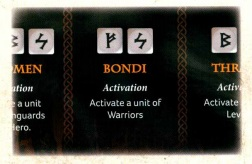
\includegraphics[width=1.0\textwidth]{pics/SagaActivationAbility} \\ \\
Способности Активаций присутствуют на каждой Боевой Доске. В основном, ты заметишь, что у тебя есть одна способность для активации своих Воинов Правителя и Геров, одна способность для активации Воинов и одна для активации Рекрутов. Цена для каждой способности отличается, и нетрудно понять, почему Рекрутов сложнее активировать, чем Воинов Правителя. В конце концов, они пришли на поле боя не по своей воле! \\ \\
Чтобы задействовать способность Активаций, сделай всё так же, как и со способностями Приказов. Просто сбрось необходимую комбинацию кубов для задействования способности и разыграй её эффект. Чтобы сбросить кубики, сними активные кубики со способности на Боевой Доске и отложи их к своим доступным кубам. Правда ведь, ничего сложного? \\ \\
Во время Фазы Активаций ты задействуешь способности Саги до тех пор, пока не решишь остановиться или пока у тебя не закончатся активные способности. 

\section*{Активация подразделений}
Задействовав способность для активации подразделения, ты должен выбрать один из четырёх вариантов активации:
\begin{itemize}
	\item Движение
	\item Атака
	\item Стрельба
	\item Отдых
\end{itemize}
Активация на движение позволяет подразделению перемещаться по полю боя (см. раздел "Движение"). \\ \\
Активация на атаку так же позволяет подразделению подвигаться, но только лишь для одной цели - встретиться с врагом в рукопашной схватке (см. раздел "Атака"). Если в ходе активации на атаку подразделение вступает в контакт с вражеским подразделением (хотя бы одна фигурка из подразделения касается базой базы фигурки из вражеского подразделения, не нарушая формации), ты должен немедленно разыграть ближний бой (см. раздел "Ближний бой"). \\ \\
Активация на стрельбу доступна только подразделениям, снаряжённым оружием дальнего боя. Активация на стрельбу позволяет таким подразделениям немедленно разыграть атаку дальнего боя против вражеского подразделения (см. раздел "Стрельба"). \\ \\
Активация на отдых требует определённых условий для выполнения, однако она позволяет подразделению восстановить свои силы, избавляясь от жетонов \textbf{усталости}, которое оно накопило (см. раздел "Отдых и усталость"). \\ \\
Дальше в этой книге ты найдёшь главы, посвящённые каждому из четырёх вариантов. \\ \\
Ты можешь активировать подразделение сколько угодно раз за Фазу Активации, до тех пор, пока у тебя есть активные способности Активаций для этого. Ты не обязан выполнять все активации одного подразделения одну за другим, - ты можешь активировать одно подразделение, затем другое, после чего вернуться к первому для новой активации. Стоит, однако, помнить, что повторные активации часто влекут за собой получение жетонов усталости. \\ \\

\subsection*{Бесплатные активации}
\begin{itemize}
	\item В правилах или описании способностей будет встречаться термин ''бесплатная активация''. Бесплатные активации - это активации, для которых не нужно задействовать способности Саги (и, следовательно, не нужно тратить свои драгоценные кубы!). Иногда вид активации строго прописан, например, ты можешь увидеть что-то вроде: ''У вашего кавалерийское подразделения есть бесплатная активация на движение''. Либо выбор вида активации будет оставлен тебе, то есть, ты увидишь что-то вроде: ''Бесплатно активируйте ваше подразделение'', и ты сможешь выбрать, совершить движение, стрельбу, атаку или отдых. Эти активации во всём остальном кроме цены кубиков Саги являются обычными активациями и подчиняются всем остальным правилам (в том числе и правилам получения усталости).
\end{itemize} 

Фаза активаций кончается когда ты больше не можешь или хочешь задействовать способности Саги. Конечно, ты можешь оставить некоторые способности активными, чтобы задействовать их в ход твоего противника ну или просто потому что не смог задействовать их в свой ход. Кубики будут терпеливо ждать своего часа. \\ \\
Как только ты решил, что твоя Фаза Активаций закончена, кончается и твой ход. \\ \\

\begingroup
\fontsize{15pt}{11pt}\selectfont
\textit{Книжник поможет тебе...}\\ \\
\fontsize{11pt}{11pt}\selectfont
\textit{Будь готов к полной событий Фазе Активаций! В отличие от других игр, в Саге нет специальной фазы для стрельбы или ближнего боя. Хочешь пострелять? Активируй подразделение и стреляй. Хочешь атаковать? Разыграй бой прямо сейчас, и, если сломил ряды противника, активируй другое подразделение, чтобы добить выживших! \\ \\
Сага предоставляет тебе огромную свободу действий, но и взимает огромную плату, если ты проведёшь свои активации в неверном порядке. Однако с опытом ты станешь отыгрывать эту фазу лучше и лучше, адаптируясь к ритму происходящего и получая огромное удовольствие от всего процесса.}
\endgroup 
\\ \\
\begingroup
\fontsize{15pt}{11pt}\selectfont
\textit{\textbf{Что ты должен запомнить}}\\ 
\fontsize{11pt}{11pt}\selectfont
\begin{itemize}
	\item Во время Фазы Активаций ты задействуешь свои способности Активаций и разыгрываешь их эффект
	\item Активированное подразделение может совершить: движение, атаку, стрельбу или отдых.
	\item Ты можешь активировать подразделение сколько угодно раз, если другие условия не препятствуют этому
	\item Твой ход заканчивается вместе с Фазой Активаций
	\item Бесплатная активация не стоит кубов Саги
\end{itemize}
\endgroup 
\newpage

\part{Движение}
\textbf{\textit{Много времени, проведённого в Саге, будет потрачено на передвижение фигурок по полю перед тем, как они смогут отправить фигурки врага к праотцам. Большинство этих перемещений являются результатом активации на движение. Правила, описывающие эти активации, просты, но строги, поэтому будь внимательнее! }}

\section*{Передвижение подразделения}

Несмотря на то, что обычно движение подразделения происходит из-за активации на движение, это не единственный способ движения для подразделения. Специальные правила, умения Саги и некоторые другие элементы игры могут заставить подразделение сменить свою позицию. Все эти движения подчиняются правилам, описанным в этой главе.

\section*{Дистанции движения}


%\addcontentsline{toc}{chapter}{5. Движение}
\part{Атака}
%\addcontentsline{toc}{chapter}{6. Атака}
\part{Стрельба}
%\addcontentsline{toc}{chapter}{7. Стрельба}
\part{Ближний бой}
%\addcontentsline{toc}{chapter}{8. Ближнр
%\addcontentsline{toc}{chapter}{9. Отдых и усталость}
\part{Особенности местности}
%\addcontentsline{toc}{chapter}{10. Особенности местности}
\part{Специальные правила}
%\addcontentsline{toc}{chapter}{11. Специальные правила}
\part{Умения Саги}
%\addcontentsline{toc}{chapter}{12. Умения Саги}
\part{Сбор отряда}
%\addcontentsline{toc}{chapter}{13. Сбор отряда}
\part{Битва Вождей}
%\addcontentsline{toc}{chapter}{14. Битва Вождей}
\part{Глоссарий}
%\addcontentsline{toc}{chapter}{Глоссарий}

\end{document}
